\FILE{hardware.tex}

\subsection{Hardware Overview}

According to the manual, FutureGrid is build out of a number of clusters of different type and size that are interconected with up to a 10GB Ethernet among its sites. The sites include Indiana University, University of Chicago, San Diego Supercomputing Center, Texas Advanced Computing Center, and University of Florida.

\subsubsection{Overview of the Clusters}\label{S:hw-cluster} 

\begin{table}[htb]

\caption{FutureGrid Compute Resources}\label{T:hw}

\begin{center}
\begin{tabular}{rrrrrrrrr}
Name    & System Type                &  \rot{Nodes} &  \rot{CPUS}   & \rot{Cores}   & \rot{TFLOPS}  & \rot{RAM (GB)}        & \rot{Storage (TB)}    & Site \\
\hline
india   & IBM iDataplex              & 128          & 256     & 1024    & 11      & 3072            & 335             & IU \\
hotel   & IBM iDataplex              & 84           & 168     & 672     & 7       & 2016            & 120             & UC \\
sierra  & IBM iDataplex              & 84           & 168     & 672     & 7       & 2688            & 96              & SDSC \\
foxtrot & IBM iDataplex              & 32           & 64      & 256     & 3       & 768             & 0               & UF \\
alamo   & Dell Poweredge             & 96           & 192     & 768     & 8       & 1152            & 30              & TACC \\
xray    & Cray XT5m                  & 1            & 166     & 664     & 6       & 1328            & 5.4             & IU \\
bravo   & HP Proliant                & 16           & 32      & 128     & 1.7     & 3072            & 128             & IU \\
delta   & \shortstack{SuperMicro\\ GPU Cluster}     & 16           & 32      & 192     &         & 1333            & 144             & IU \\
lima    & Aeon Eclipse64             & 8            & 16      & 128     & 1.3     & 512             & 3.8             & SDSC \\
echo    & \shortstack{SuperMicro \\ScaleMP Cluster} & 16           & 32      & 192     & 2       & 6144            & 192             & IU \\
\end{tabular}
\end{center}
\end{table}


\begin{sidewaystable}

\caption{FutureGrid cluster details.}\label{F:cluster-details}
~\\
\begin{footnotesize}
\begin{tabular}{|p{2cm}||p{4cm}p{1.5cm}p{1.5cm}p{1.5cm}p{1.5cm}p{1.5cm}p{1.5cm}p{1.5cm}p{1cm}|}
\hline
 \bf Name                                & \bf Echo & \bf Alamo & \bf Bravo & \bf Delta & \bf Foxtrot & \bf Hotel & \bf India & \bf Sierra & \bf Xray \\
\hline
\hline
 Organization                        & IU & TACC & IU & IU & UF & UC & IU & SDSC & IU \\
\hline
 Machine Type                        & Cluster SclaeMP & Cluster & Cluster & Cluster & Cluster & Cluster & Cluster & Cluster & Cluster \\
\hline
 System Type                         &SuperMicro& Dell PowerEdge M610 Blade & HP Proliant && IBM iDataPlex dx 360 M2 & IBM iDataPlex dx 360 M2 & IBM iDataPlex dx 360 M2 & IBM iDataPlex dx 340 & Cray XT5m \\
\hline
 CPU Type                            & Xeon E5-2640 &  Xeon X5550 &  Xeon E5620 &  Xeon 5660 &  Xeon X5520 &  Xeon X5550 &  Xeon X5550 &  Xeon L5420 & Opteron 2378 \\
\hline
 CPU Speed                           &2.50GHz& 2.66GHz & 2.40GHz & 2.80 GHz & 2.26GHz & 2.66GHz & 2.66GHz & 2.5GHz & 2.4GHz \\
\hline
 CPUs                                &&192&32&32&64&168&256&168&168 \\
\hline
 Servers                             &12&96&16&16&32&84&128&84&1 \\
\hline
 RAM                                 && 12GB DDR3 1333Mhz & 192GB DDR3 1333Mhz & 192GB DDR3 1333 Mhz & 24GB DDR3 1333Mhz & 24GB DDR3 1333Mhz & 24GB DDR3 1333Mhz & 32GB DDR2-667 & 8GB DDR2-800 \\
\hline
 Total RAM                           &&1152GB&3072GB&3072GB&768GB&2016GB&3072GB&2688GB&1344GB \\
\hline
 Number of cores                     &144&768&128&&256&672&1024&672&672 \\
\hline
 Tflops                              &&8&1.7&&3&7&11&7&6 \\
\hline
 Disk Size (TB)                      &2.8&48&&15&20&120&335&72&335 \\
\hline
 Hard Drives                         && 500GB 7.2K RPM SAS & 6x2TB 7.2K RPM SATA & 92GB 7.2K RPM SAS2 & 500GB 7200 RPM SATA & 1 TB 7200 RPM SATA & 3000GB 7200 RPM SATA & 160GB 7200 RPM SATA Drive & 6TB Lustre \\
\hline
 Shared Storage                      && NFS & NFS &NFS& NFS & GPFS & NFS & ZFS 82.2TB & NFS \\
\hline
 Interconnect                        && Mellanox 4x QDR IB & Mellanox 4x DDR IB &&& Mellanox 4x DDR IB & Mellanox 4x DDR IB & Mellanox 4x DDR IB & Cray SeaStar \\
\hline
\end{tabular}
~\\
IB = InfiniBand, Xenon = INtel Xenon, Opteron = AMD Opteron 

\end{footnotesize}

\end{sidewaystable}



\subsubsection{Overview of Networking}

The significant number of distinct systems within FutureGrid provide a
heterogeneous distributed architecture and are connected by
high-bandwidth network links supporting distributed system research
\cite{las12fg-bookchapter}. FutureGrids network used to have a
dedicated network between sites \cite{las12fg-bookchapter}. However,
the network infrastructure has recently changed due to changes as part
of its major network operator the National Lambda Rail.  Due to these
changes the operation of the network between the sites conducted by
the national lambda rail has switched opertaion to XSEDE and are no
longer exclusive. This is no major handicap for the projects conducted
on FutureGrid based on our project portfolio.  The current high level
network diagram is depicted in Figure~\ref{F:network}.

The core resources to FutureGrid at SDSC, IU, TACC, and UF are now all
connected via the XSEDE network and integrated via the FG core router
in Chicago. WIthin The IU network additional clusters are integrated
and are described in more detail in Section~\ref{S:hw-cluster}. 

A Spirent H10 XGEM Network Impairment emulator
\cite{www-network-impairment} can be colocated with resources at
Indiana University, to enable experiments to include network latency,
jitter, loss, and errors to network traffic.

In addition we have added several shaded components that are related
to a spcial software service called cloudmesh that we explain in more
detail in Section~\ref{S:cloudmesh}.


\begin{figure}[htb]
  \centering
    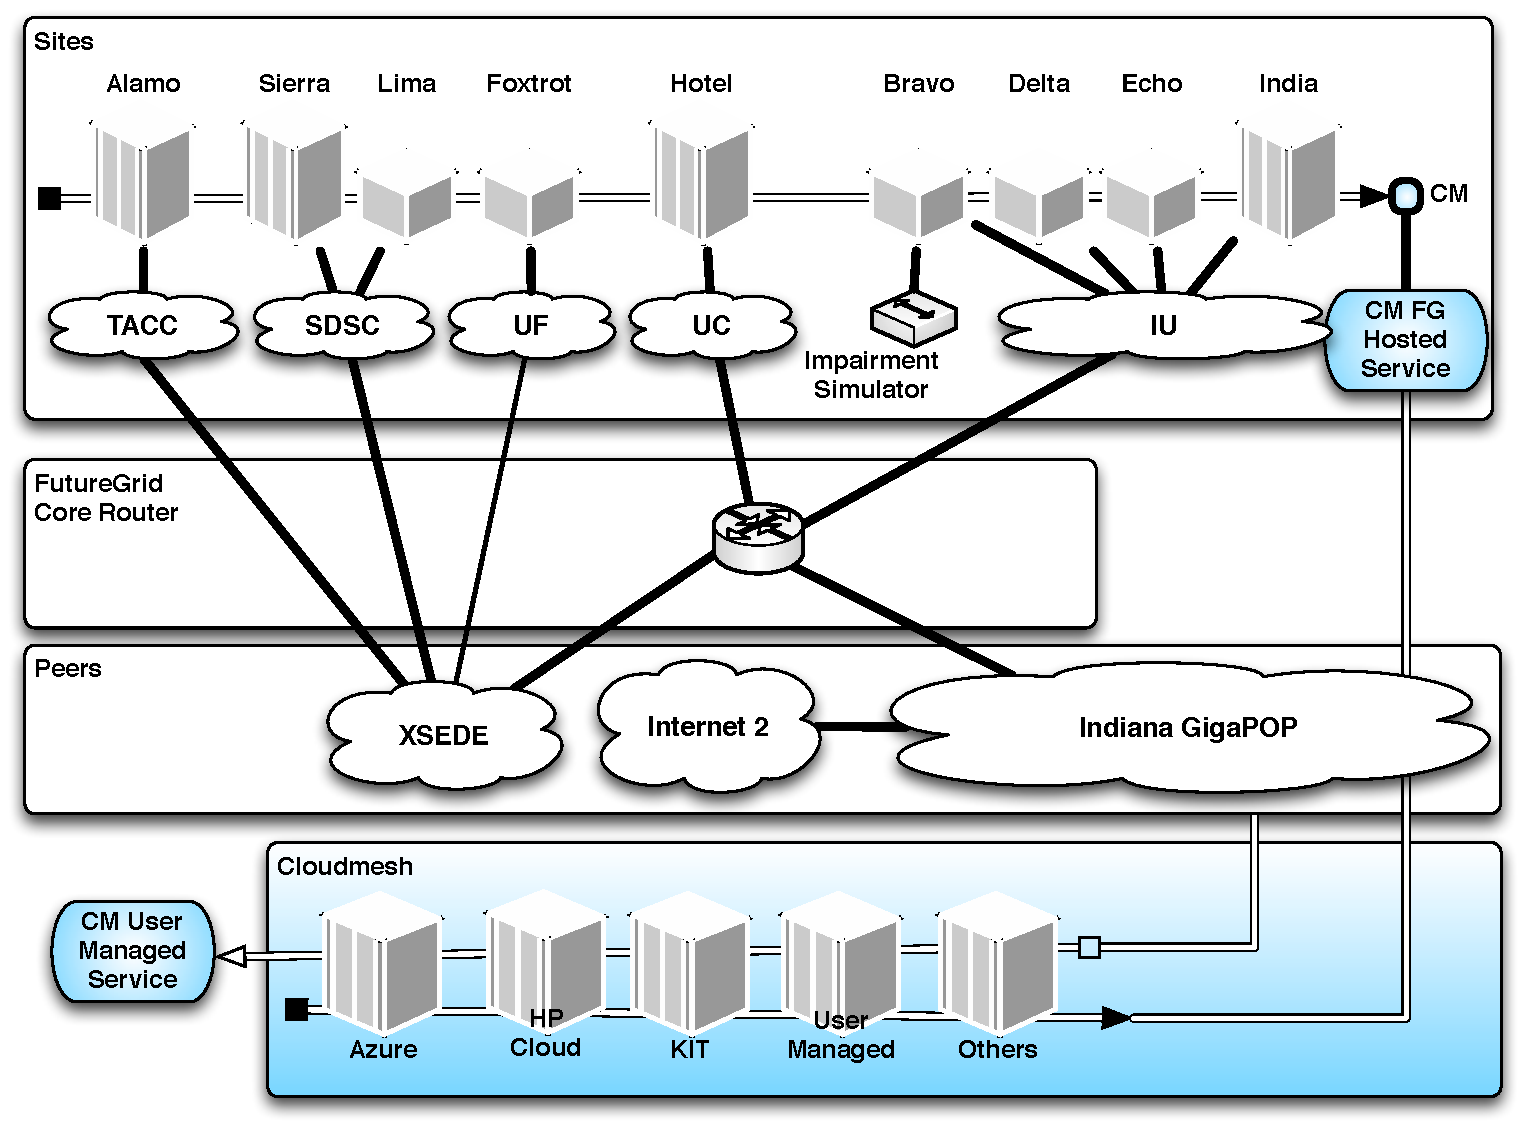
\includegraphics[width=1.0\textwidth]{images/fg-network-2014-cm.pdf}
  \caption{High level network diagram and conceptual integration of cloudmesh resources.}
\label{F:network}
\end{figure}

\subsubsection{Overview of Storage}

FutureGrid has only a very limited amount of storage space and users
are requested to remove their storage space after use. GutureGrid does
not provide capacity for long term storage or long term
experiments. Users with special needs may be acomodated by special
storage setups. The list of storage services is shown in Table \ref{T:storage}.

\begin{table}[htb]
\caption{Storage Resources of FutureGrid.}
\label{T:storage} 

\centering{}%
\begin{tabular}{lrll}
\textbf{System Type } & \textbf{Capacity(TB) } & \textbf{File System } & \textbf{Site }\tabularnewline
\hline 
Xanadu 360  & 180  & NFS  & IU \tabularnewline
DDN 6620  & 120  & GPFS  & UC \tabularnewline
Sunfire x4170  & 96  & ZFS  & SDSC \tabularnewline
Dell MD3000  & 30  & NFS  & TACC \tabularnewline
IBM dx360 M3  & 24  & NFS  & UF \tabularnewline
\end{tabular}
\end{table}

